\section{Versuchsaufbau}
\label{versuchsaufbau}

Generelle Netzstruktur, softmax auf Klassen abgebildet
Conv mit MaxPool gefolgt von AveragePool auf Fully Connect auf Softmax

\subsection{Datensätze}
\label{datensaetze}

\paragraph{MNIST}
\label{mnist}

\emph{\gls{MNIST}} Datensatz

Bei den Datensätzen insbesondere auch die Superpixelalgorithmen erwähnen
das heißt wie viele Superpixel
welche Parameter
mean/max Knotengrad
Wie viele Merkmale und welche?

\cite{mnist}

\section{MNIST}

Trainingsbilder: 55.000

\begin{itemize}
  \item 10.000 Steps mit Batch Size 64 (ungefähr 12 Epochen)
  \item Learning Rate 0.001
  \item klassisches Convolution Neural Network nachgebildet mit Gridgraphen
  \item Conv1: $5 \times 5$, $1 \rightarrow 32$
  \item MaxPool1: Size 2, Stride 2
  \item Conv2: $5 \times 5$, $32 \rightarrow 64$
  \item MaxPool2: Size 2, Stride 2
  \item FC1: 1024
  \item Dropout: 0.5
  \item FC2: 10
\end{itemize}

\subsection{Auswertung}

\begin{itemize}
  \item \textbf{2D Conv > Max:} 0.18s pro Batch, Accuracy: 99.189, Cost: 0.03458
  \item \textbf{2D Conv > 2D Conv > Max:} 0.25s pro Batch, Accuracy: 99.139, Cost: 0.03062
  \item \textbf{Chebyshev $k=25$ GCNN:} 0.91s pro Batch, Accuracy: 98.888, Cost: 0.04329
  \item \textbf{$k=1$ GCNN:} 0.22s pro Batch, Accuracy: 96.765, Cost: 0.10596
  \item \textbf{Partitioned GCNN:}
  \begin{itemize}
    \item Conv > Max: 0.45s pro Batch, Accuracy: 98.998, Cost: 0.03198
    \item Conv > Conv > Max: 2.87s pro Batch, Accuracy: 99.189, Cost: 0.02704
  \end{itemize}
\end{itemize}

\subsection{SLIC}

\begin{itemize}
  \item keine lokale Normierung
  \item Stddev: $1$
  \item 4 Level
  \item Graphkonnektivität: $1$
  \item Anzahl Segmente: $100$
  \item Compactness: $10$
  \item Maximum Iterations: $10$
  \item Sigma: $0$
  \item Anzahl Partitionen: 8
  \item Features: Area, Bbox height, bbox width, Mean Color = $4$ Features
  \item \textbf{Aufbau}: Conv zu 32, Pool2, Conv zu 64, Pool2, Conv zu 128, Pool2, Conv zu 256, Pool2, AveragePool, FC210
  \item Meiste zeit wird durch Partitionierung verschwendet.
  \item \textbf{Ergebnisse}: 0.79s pro Batch, Accuracy: 0,79497, Loss: 0.62814
  \item enttäuschend!
\end{itemize}

\section{PascalVOC}

erster Test:
17 s Preprocess, 12s Training auf BatchSize 64
loss = 0.2, acc = 0.55


\paragraph{CIFAR-10}
\label{cifar_10}

\cite{cifar_10}

Der \emph{\gls{Cifar}} Datensatz
Er liegt in zwei Versionen vor, \gls{Cifar}-10 und \gls{Cifar}-100, wobei sich diese Arbeit an dem weitaus beliebteren Datensatz \gls{Cifar}-10 bedient.

\begin{figure}[t]
\centering
\subfigure[\gls{SLIC}]{%
  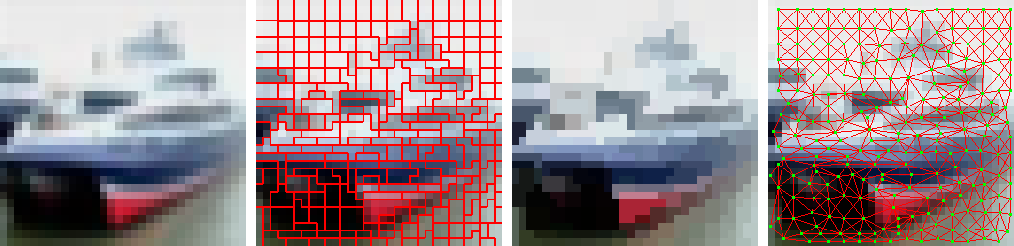
\includegraphics[width=\textwidth]{bilder/cifar_10_slic.png}
}
\subfigure[Quickshift]{%
  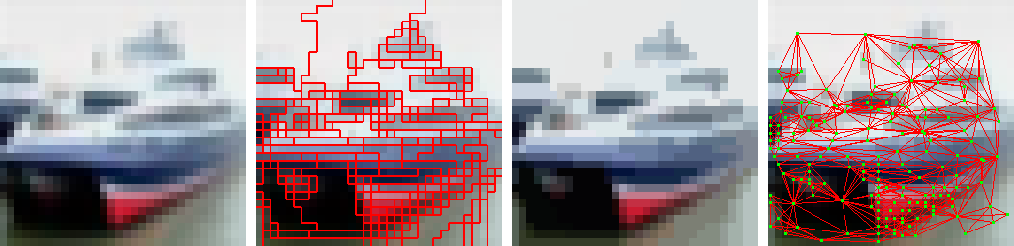
\includegraphics[width=\textwidth]{bilder/cifar_10_quickshift.png}
}
  \caption[\gls{Cifar}-10]{Bild des \gls{Cifar}-10 Datensatzes~\cite{cifar_10}, jeweils dargestellt als (1) Originalbild, (2) Superpixelrepräsentation, (3) Durchschnittsfarbe der Superpixel und (4) Graphrepräsentation.}
\label{fig:cifar_10}
\end{figure}


% \paragraph{Tiny ImageNet}
% \label{tiny_image_net}

% \cite{imagenet}

\paragraph{PASCAL VOC}
\label{pascal_voc}

\emph{\gls{Pascal}} Datensatz
\cite{pascal_voc}

\begin{figure}[t]
\centering
\subfigure[\gls{SLIC}]{%
  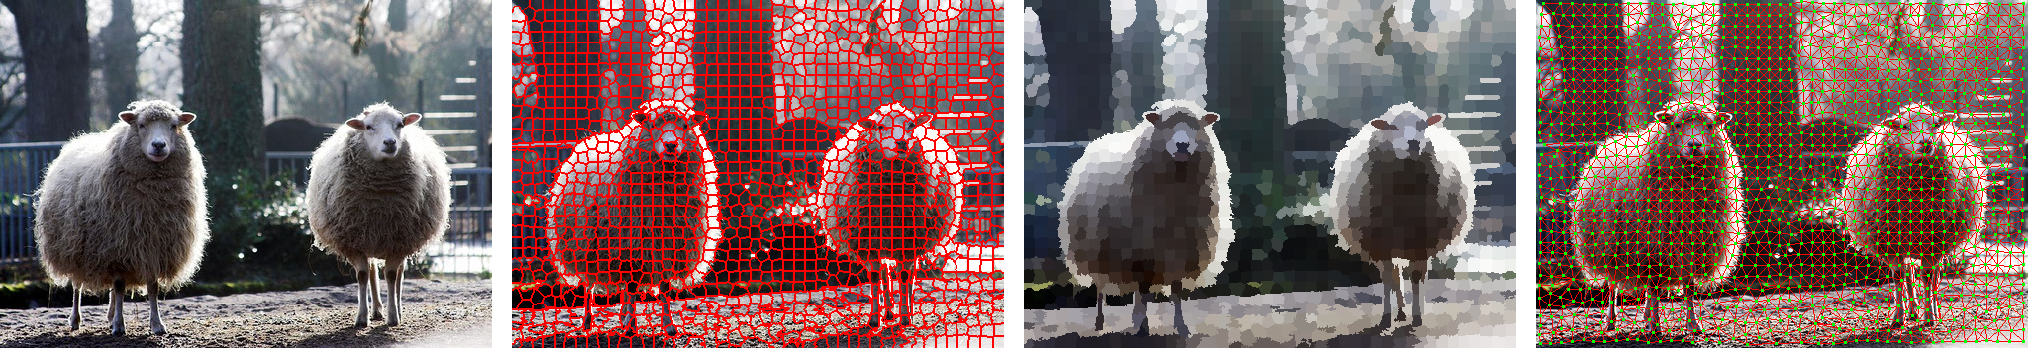
\includegraphics[width=\textwidth]{bilder/pascal_voc_slic.png}
}
\subfigure[Quickshift]{%
  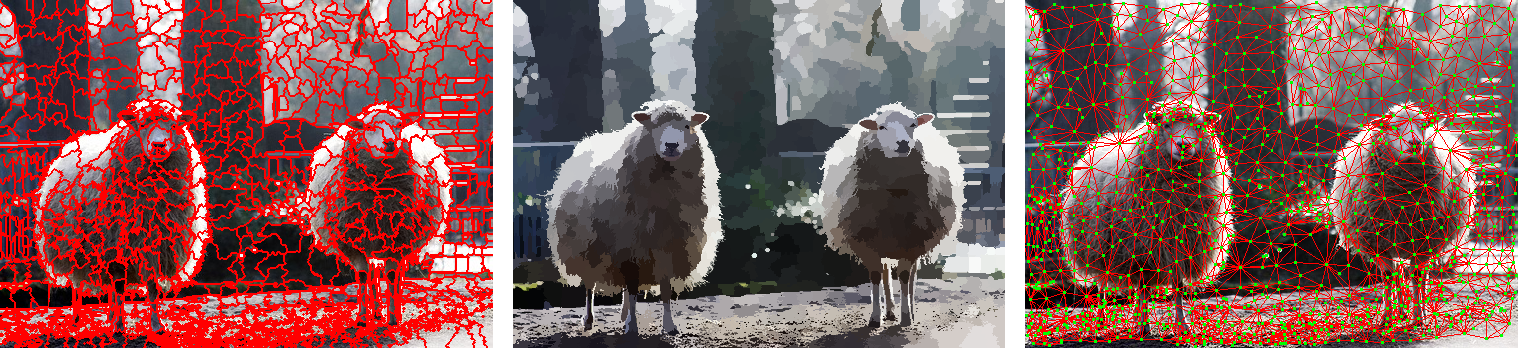
\includegraphics[width=\textwidth]{bilder/pascal_voc_quickshift.png}
}
  \caption[\gls{Pascal}]{Bild des \gls{Pascal} Datensatzes~\cite{pascal_voc}, jeweils dargestellt als (1) Originalbild, (2) Superpixelrepräsentation, (3) Durchschnittsfarbe der Superpixel und (4) generierter Graph.}
\label{fig:pascal_voc}
\end{figure}


\subsection{Metriken}
\label{metriken}

\subsection{Parameterwahl}
\label{parameterwahl}

Vorstellung aller Parameter
Was gibt es denn hier überhaupt?
Dropout, L2 Regularisierung?
BatchSize?
Globale/normale Lokalisierung
Standardabweichung für Gauß

Alle Faltungen wurden dabei mit einer Partitionsgröße von $8$ bei $K=0$ und $K=1$ implementiert, um ein \gls{CNN} mit einem $3 \times 3$ Filter zu simulieren.
Es erscheint jedoch vorstellbar die Filtergröße bei größerer lokaler Kontrollierbarkeit, \dhe{} $K > 1$, weiter zu reduzieren und die Gefahr des Overfittings damit aufgrund der kleineren Anzahl an Trainingsparametern einzuschränken.

\paragraph{Datenreduktion}
\label{datenreduktion}

\subsection{Augmentierung von Graphen}
\label{augmentierung_von_graphen}

hier auf die Formeln von TensorFlow referenzieren, d.h. TensorFlow Quelle angeben
\cite{tensorflow}

Augmentierung auf Graphen über left/right
Farbanpassungen


nesser ist es, dass Bild vorher zu ändern, da sich dadurch die Superpixelrepräsentation ändert
und folglich zu realisiterischer Augmentierung führt.

\subsection{Vorverarbeitung und Eingabe der Daten}
\label{vorverarbeitung}
